\documentclass{beamer}
\include{graphicsx}
\title{Hacking Protrekkr}
\author{Paul Batchelor}

\begin{document}

\begin{frame}
\maketitle
\end{frame}

\begin{frame}
\frametitle{What is Protrekkr?}
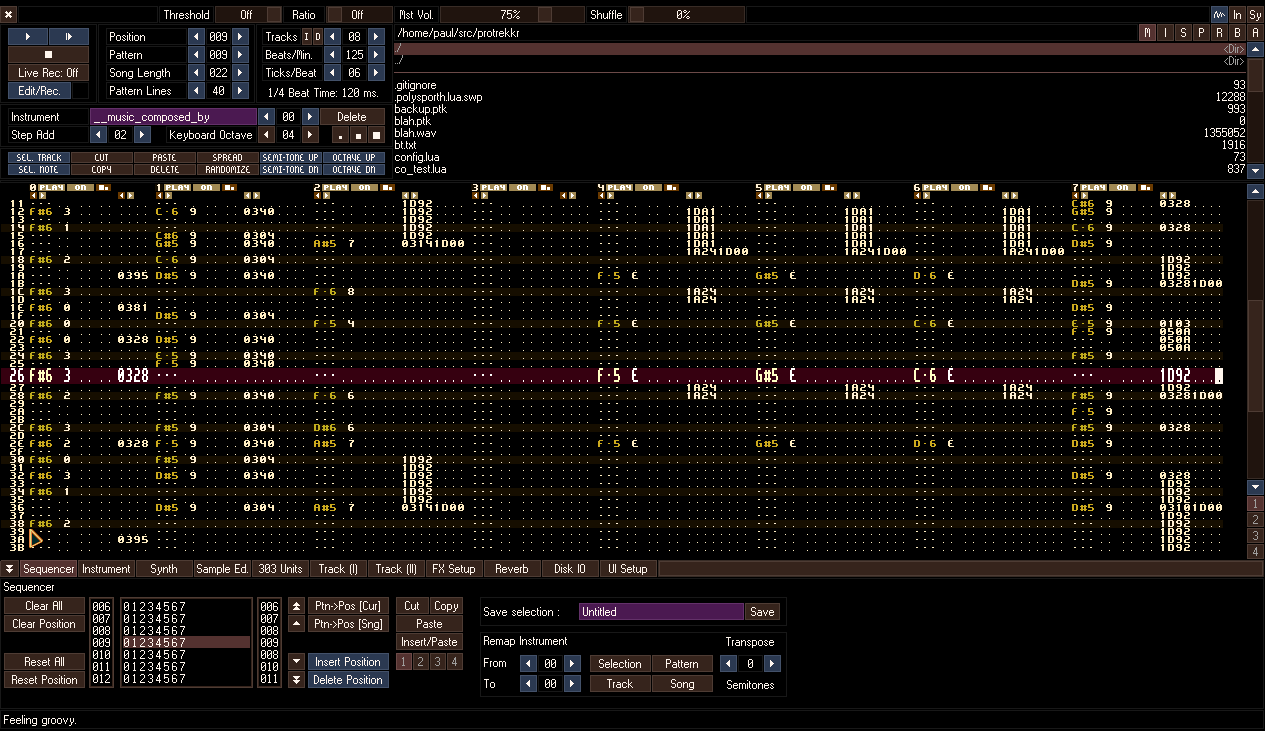
\includegraphics[scale=0.25]{../ptk}
\end{frame}

% \begin{frame}
% \frametitle{What is Protrekkr?}
% 
% \begin{itemize}
%     \item{Music software originally by Arguru}
%     \item{Multi-platform (Linux, Windows, Mac, Amiga, AROS, PSP, etc..)}
%     \item{Free Open Source Software}
%     \item{Dead project}
%     \item{...ripe for hacking!}
% \end{itemize}
% 
% \end{frame}

\begin{frame}

\frametitle{Protrekkr is a music tracker}
\begin{itemize}
    \item{Popular interface for music production in the 80s and 90s}
    \item{Kind of looks like a spreadsheet?}
    \item{Time moves top/bottom instead of left/right}
    \item{Rows denote equal divisions of time}
    \item{Columns denote instruments/notes/tracks}
    \item{Typically sample-based}
    \item{There are a *lot* of music trackers...}
\end{itemize}

\end{frame}

\begin{frame}
\frametitle{DMC (Commodore 64)}
\begin{center}
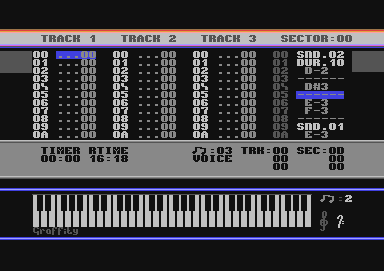
\includegraphics[scale=0.5]{dmc}
\end{center}
\end{frame}

\begin{frame}
\frametitle{AHX (Amiga)}
\begin{center}
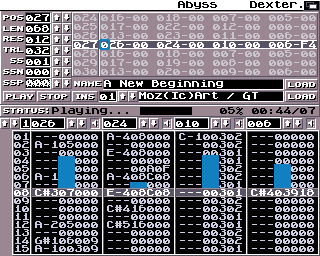
\includegraphics[scale=0.6]{ahx}
\end{center}
\end{frame}

\begin{frame}
\frametitle{Impulse Tracker (DOS)}
\begin{center}
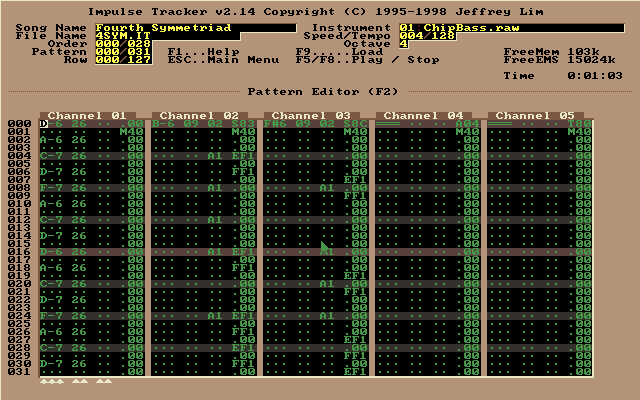
\includegraphics[scale=0.4]{impulsetracker}
\end{center}
\end{frame}

\begin{frame}
\frametitle{Fasttracker (DOS)}
\begin{center}
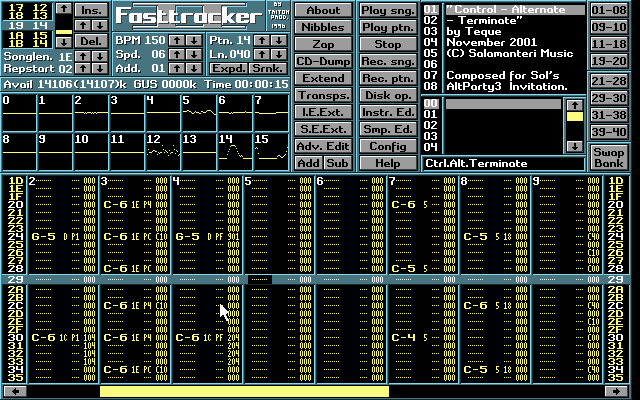
\includegraphics[scale=0.4]{fasttracker}
\end{center}
\end{frame}

\begin{frame}
\frametitle{LSDJ (Gameboy)}
\begin{center}
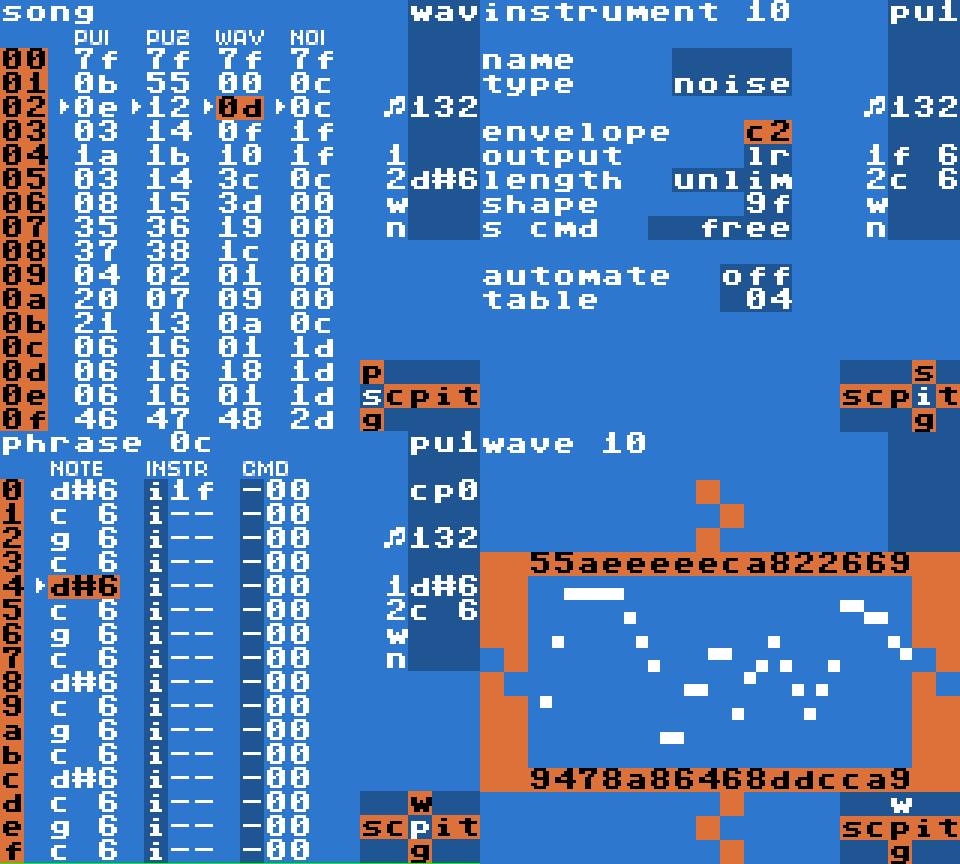
\includegraphics[scale=0.2]{lsdj}
\end{center}
\end{frame}

\begin{frame}
\frametitle{Sunvox (Linux/Mac/Windows/Android/iOS)}
\begin{center}
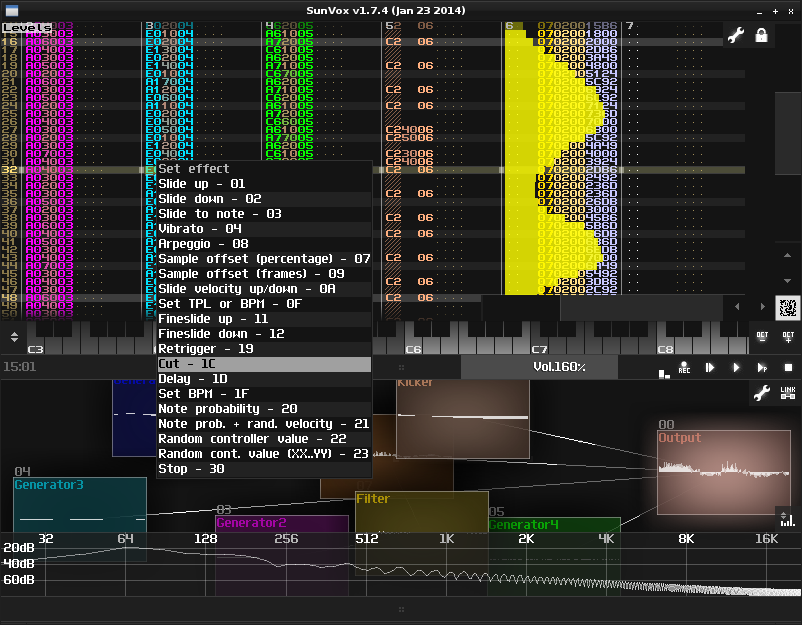
\includegraphics[scale=0.3]{sunvox}
\end{center}
\end{frame}

\begin{frame}
\frametitle{Renoise (Linux/Mac/Windows)}
\begin{center}
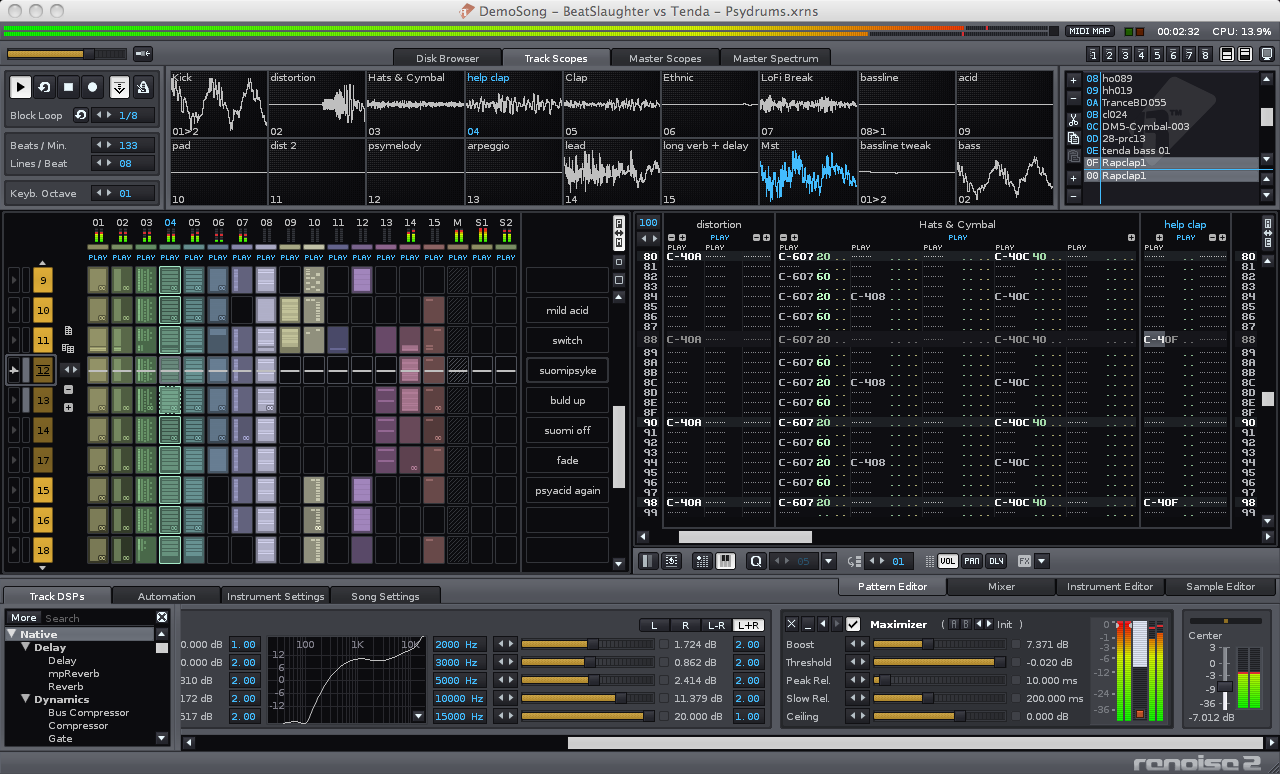
\includegraphics[scale=0.2]{renoise}
\end{center}
\end{frame}

\begin{frame}
\frametitle{Milkytracker (Linux/Mac/Windows/Android/iOS)}
\begin{center}
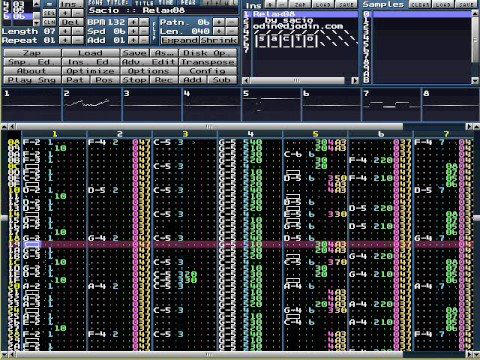
\includegraphics[scale=0.5]{milkytracker}
\end{center}
\end{frame}

\begin{frame}
\frametitle{Goattracker (Linux/Mac/Windows)}
\begin{center}
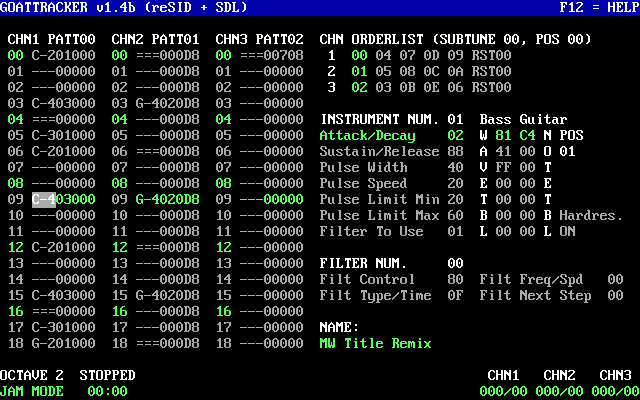
\includegraphics[scale=0.4]{goattracker}
\end{center}
\end{frame}

\begin{frame}
\frametitle{Radium (Linux/Mac/Windows)}
\begin{center}
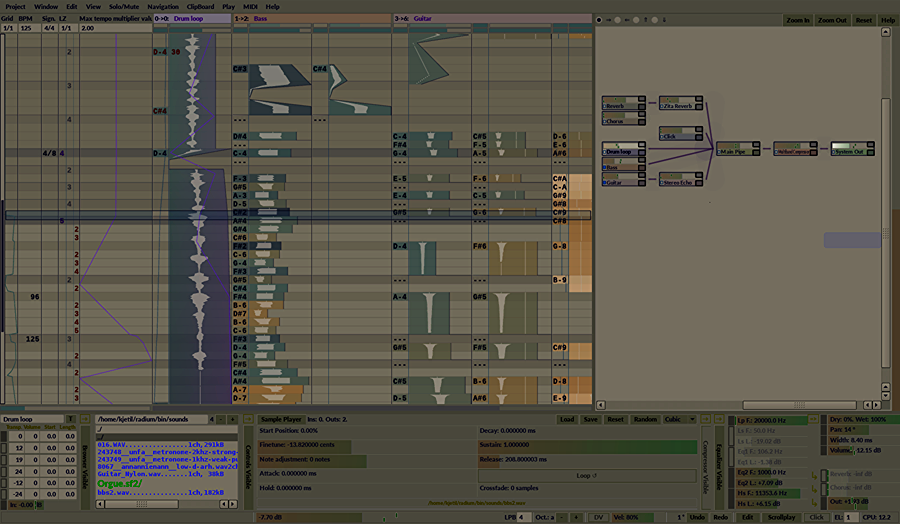
\includegraphics[scale=0.3]{radium}
\end{center}
\end{frame}

\begin{frame}
\frametitle{Famitracker (Windows)}
\begin{center}
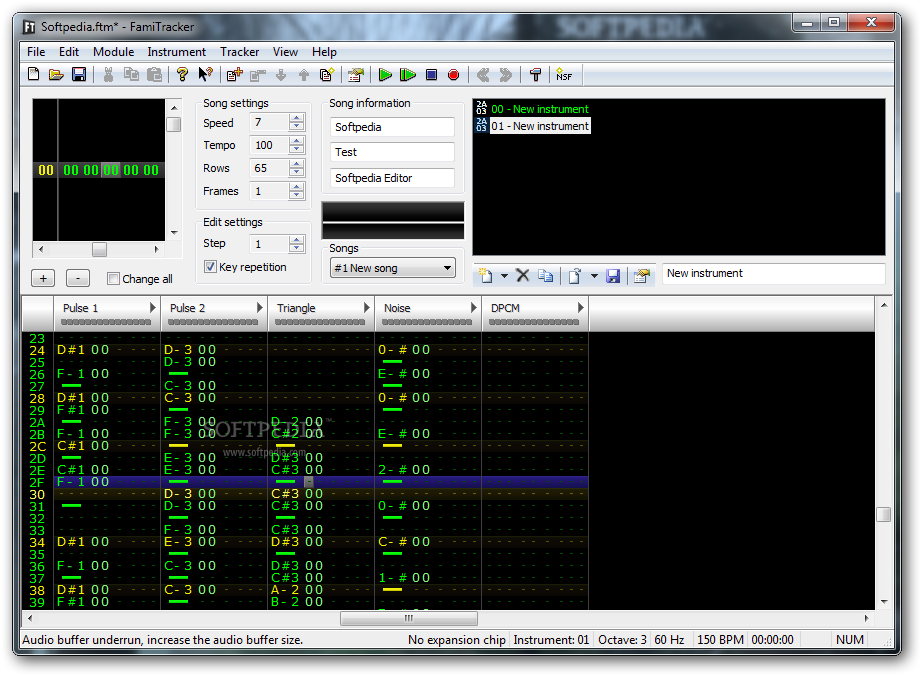
\includegraphics[scale=0.4]{famitracker}
\end{center}
\end{frame}

\begin{frame}
\frametitle{and several others...}
\begin{itemize}
    \item{Jeskola Buzz}
    \item{Modplug}
    \item{Schism}
    \item{Psycle}
    \item{Klystrack}
    \item{Adlib Tracker 2}
    \item{Soundtracker}
    \item{Cheesetracker}
    \item{OpenMPT}
\end{itemize}

\end{frame}

\begin{frame}
\frametitle{Why Protrekkr?}
\begin{itemize}
    \item{Made for more modern computers}
    \item{Out-of-the-box JACK support (Linux)}
    \item{Built in wavetable synthesizer}
    \item{Signal processing: compressors, EQ, filters, Reverb}
    \item{Two programmable tb303 units}
\end{itemize}

\end{frame}

\begin{frame}
\frametitle{New Features Added}
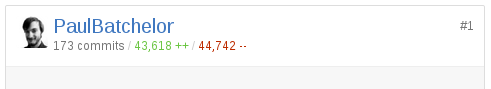
\includegraphics[scale=0.3]{git}
\begin{itemize}
    \item{Refactoring}
    \item{Lua Scripting}
    \item{Sporth + live coding server}
\end{itemize}
\end{frame}

\begin{frame}
\frametitle{Future features?}
\begin{itemize}
    \item{Define an API}
    \item{ptk file player}
    \item{Custom Widgets}
    \item{OSC support}
\end{itemize}
\end{frame}

\begin{frame}
\frametitle{More info}
\begin{itemize}
    \item{Project Page: pbat.ch/proj/protrekkr}
    \item{Github: www.github.com/paulbatchelor/protrekkr.git}
\end{itemize}
\end{frame}

\end{document}
